\documentclass{standalone}
\usepackage{PhysicalChemistryNote}
\begin{document}
\begin{tikzpicture}
    \draw[-] (0,0) -- (4,0);
    \draw[->] (0,0) -- (0,4.25) node[left]{$p$};
    \draw[-] (4,0) -- (4,4);
    \draw[-] (0,4) -- (4,4);
    \node[below] at (0,0) {$B$};
    \node[below] at (4,0) {$A$};
    \node[below] at (2,0) {$x_{A,\g}$};
    \draw[domain=0:4] plot[smooth](\x,{4*1.25*2.75/(11-1.5*\x)});
    \filldraw[fill=lightgray,opacity=0.5,domain=0:4] plot[smooth](\x,{4*1.25*2.75/(11-1.5*\x)}) -- (4,4) -- (0,4);
    \filldraw[fill=violet,opacity=0.1,domain=0:4] plot[smooth](\x,{4*1.25*2.75/(11-1.5*\x)}) -- (4,0) -- (0,0);
    \node[left] at (0,1.25) {$p_B^\ast$};
    \node[right] at (4,2.75) {$p_A^\ast$};
    \node[below] at (2,1.5) {\small{$\dfrac{p_A^\ast p_B^\ast}{p_A^\ast+\left(p_B^\ast-p_A^\ast\right)x_{A,\g}}$}};
    
    
\end{tikzpicture}
\end{document}